\documentclass{beamer}
\usefonttheme[onlymath]{serif}

\usepackage[utf8]{inputenc}
\usepackage[T1]{fontenc}
\usepackage{lmodern}
\usepackage[francais]{babel}

% For table
\usepackage{booktabs} % To thicken table lines
\usepackage{multirow}
\usepackage{amsmath,amssymb,amsfonts}

\graphicspath{{img/}}

\usepackage{cite}
\usepackage{graphicx}
\usepackage{textcomp}
\usepackage{xcolor}
\usepackage[group-separator={,}]{siunitx}
\def\BibTeX{{\rm B\kern-.05em{\sc i\kern-.025em b}\kern-.08em
		T\kern-.1667em\lower.7ex\hbox{E}\kern-.125emX}}

\usepackage{booktabs} %top/mid/bottom rule

\definecolor{red}{RGB}{255,0,0}
\definecolor{green}{RGB}{0, 102, 0}
\definecolor{maron}{RGB}{102,51,0}
\definecolor{orange}{RGB}{255,128,0}
\definecolor{blue}{RGB}{0,153,153}


\mode<presentation> {
	\usetheme{ulaval}
	\setbeamercovered{invisible}
}

\logo{
	
\includegraphics[height=0.65cm, keepaspectratio]{graal.pdf}\hspace{.2cm}\vspace{.85\paperheight}}


\title{Leveraging Subword Embeddings for Multinational Address Parsing}

\author[Yassine et al.]{Marouane Yassine, David Beauchemin, \\ François Laviolette, Luc Lamontagne}
\institute[Université Laval]
{
	Département d'informatique et de génie logiciel, \\
	Université Laval\\
	\medskip
	{\emph{marouane.yassine.1@ulaval.ca, david.beauchemin.5@ulaval.ca, francois.laviolette@ift.ulaval.ca, luc.lamontagne@ift.ulaval.ca}}
}
\date{July 14 2020}

\AtBeginSection[]
{
	\begin{frame}<beamer>
		\frametitle{Agenda}
		\tableofcontents[currentsection]
	\end{frame}
}

\begin{document}
	
	\begin{frame}[label=titre, plain]
		\titlepage
		\begin{center}
			
\includegraphics[height=1cm]{graal}
			
\includegraphics[height=1cm]{UL_P}
		\end{center}
	\end{frame}
	
	\section{Introduction}
	
	\begin{frame}{Introduction}
		...
	\end{frame}

	\section{Related Work}
	\begin{frame}{Related Work}
		...
	\end{frame}

	\section{Subword Embeddings}
	\begin{frame}{Subword Embeddings}
		...
	\end{frame}

	\section{Architecture}
	\begin{frame}{Architecture}
		\begin{figure}[h!]
			\centering
			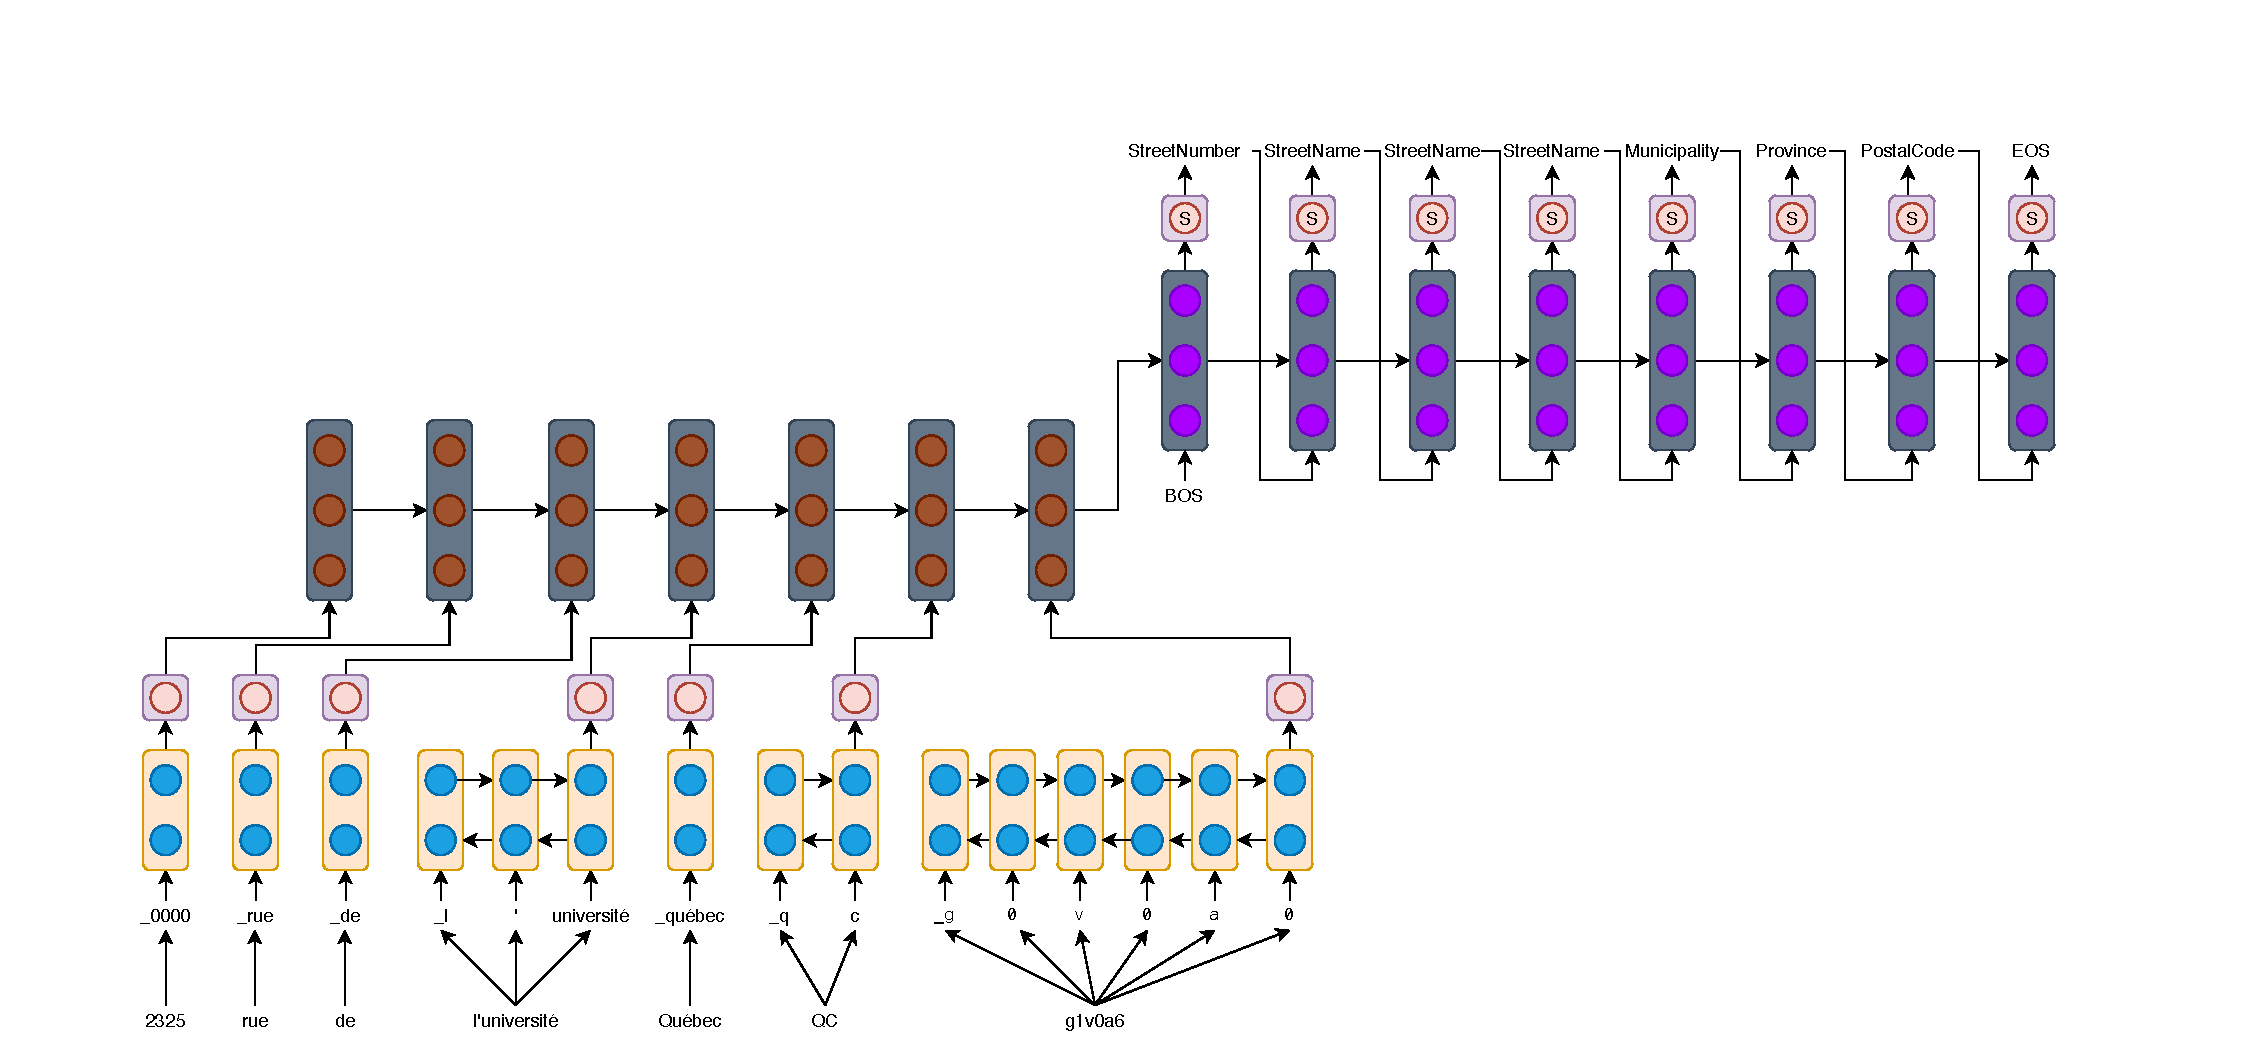
\includegraphics[width=1.1\textwidth,height=\textheight,keepaspectratio]{Network.pdf}
		\end{figure}
	\end{frame}
	
	\section{Data}
	\begin{frame}{About the Data}
		\begin{figure}[h!]
			\centering
			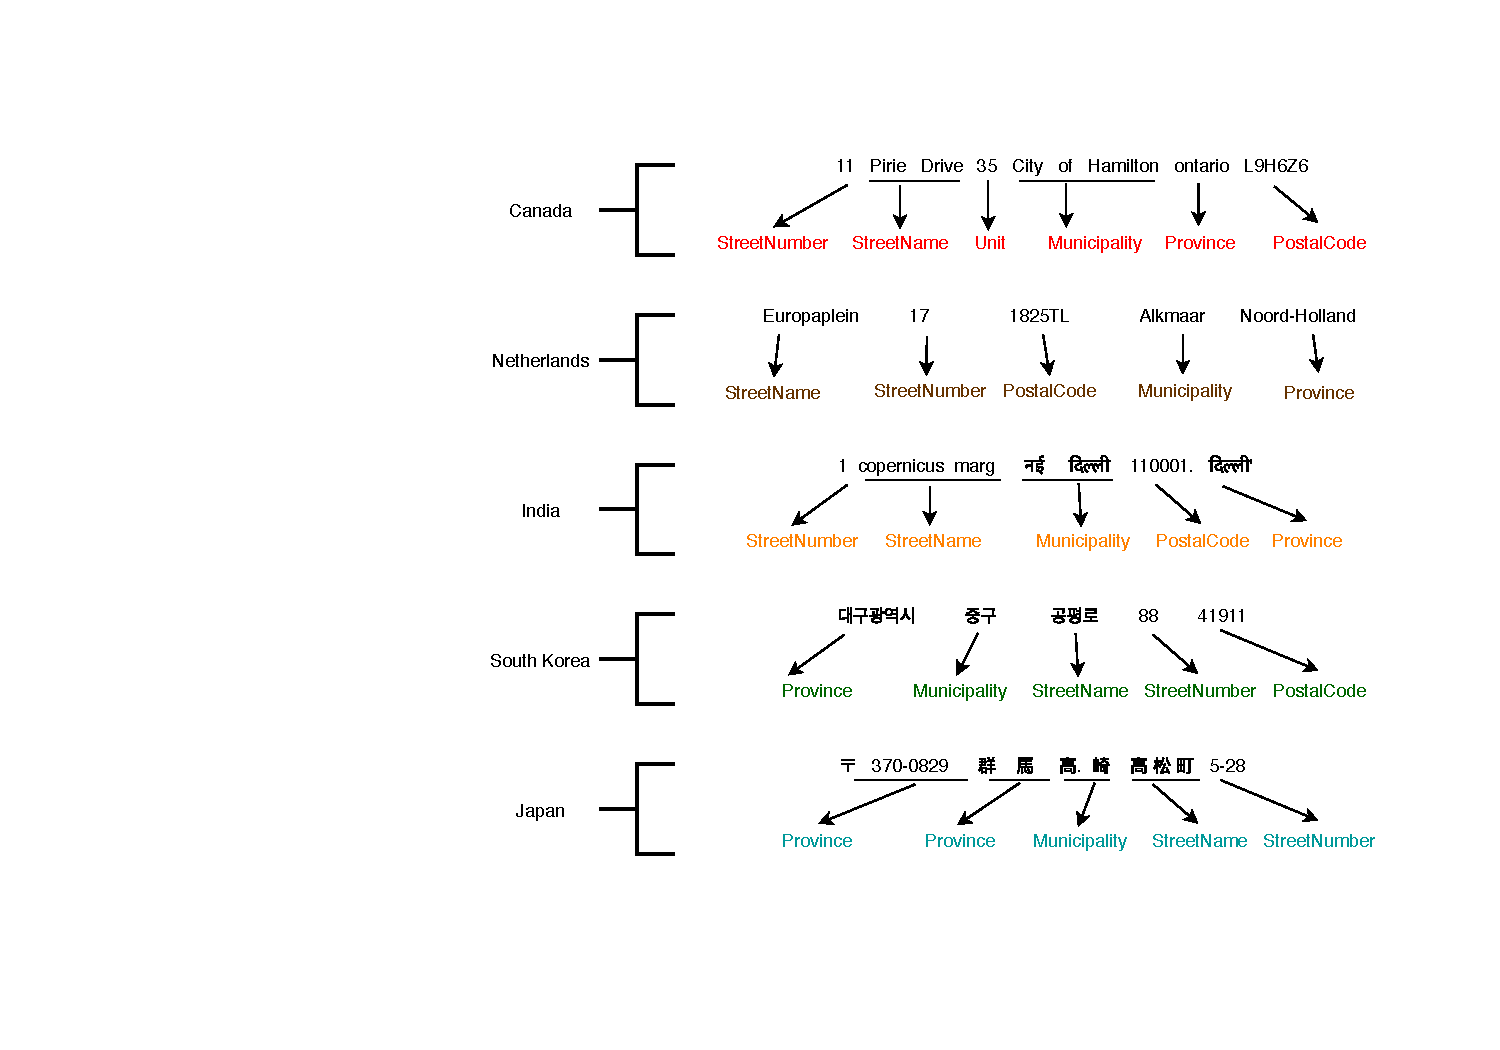
\includegraphics[width=0.8\textwidth,height=0.8\textheight,keepaspectratio]{Samples2.pdf}
		\end{figure}
	\end{frame}

	\begin{frame}{Training Data}
		100K of each country ...
	\end{frame}

	\begin{frame}{Holdout Test Set}
		\resizebox{\textwidth}{!}{%
			\begin{tabular}{cccccccc}
				\toprule
				Country & Number of samples & Country & Number of samples & Country & Number of samples & Country & Number of samples \\ \midrule
				\color{red}United States & \num{8000000} & \color{maron}Germany & \num{1576059} & \color{maron}Poland & \num{459522} &  \color{maron}Czechia & \num{195269} \\ 
				\color{red}Brazil & \num{8000000} & \color{maron}Spain & \num{1395758} & \color{maron}Norway & \num{405649} & \color{maron} Italy & \num{178848} \\ 
				\color{green}South Korea & \num{6048106} & \color{maron}Netherlands & \num{1202173} & \color{maron}Austria & \num{335800} &  \color{maron}France & \num{20050} \\ 
				\color{red}Australia & \num{5428043} & \color{red}Canada & \num{910891} & \color{maron}Finland & \num{280219} &  \color{red}United Kingdom & \num{14338} \\ 
				\color{maron}Mexico & \num{4853349} & \color{maron}Switzerland & \num{474240} & \color{maron}Denmark & \num{199694} &  \color{red}Russia & \num{8115} \\
				\bottomrule
			\end{tabular}%
		}	
	\end{frame}

	\begin{frame}{Zero-Shot Test Set}
		\resizebox{\textwidth}{!}{%
		    \begin{tabular}{cccccccc}
				\toprule
				Country & Number of samples & Country & Number of samples & Country & Number of samples & Country & Number of samples \\ \midrule
				\color{maron}Belgium & \num{66182} & \color{maron}Slovenia & \num{9773} & \color{maron}Réunion & \num{2514} &  \color{red}Singapore & \num{968} \\ 
				\color{maron}Sweden & \num{32291} & \color{red}Ukraine & \num{9554} & \color{maron}Moldova & \num{2376} &  \color{red}Bangladesh & \num{888} \\ 
				\color{maron}Argentina & \num{27692} & Belarus & \num{7590} & \color{red}Indonesia & \num{2259} &  \color{maron}Paraguay & \num{839} \\ 
				\color{orange}India & \num{26084} & \color{maron}Serbia & \num{6792} & \color{red}Bermuda & \num{2065} &  \color{maron}Cyprus & \num{836} \\ 
				\color{maron}Romania & \num{19420} & \color{maron}Croatia & \num{5671} & \color{maron}Malaysia & \num{2043} &  \color{maron}Bosnia & \num{681} \\ 
				\color{maron}Slovakia & \num{18975} & \color{maron}Greece & \num{4974} & \color{red}South Africa & \num{1388} &  \color{red}Ireland & \num{638} \\ 
				Hungary & \num{17460} & \color{red}New Zealand & \num{4678} & \color{red}Latvia & \num{1325} &  \color{maron}Algeria & \num{601} \\ 
				\color{blue}Japan & \num{14089} & \color{maron}Portugal & \num{4637} & \color{blue}Kazakhstan & \num{1087} &  \color{maron}Colombia & \num{569} \\ 
				\color{red}Venezuela & \num{10696} & \color{maron}Lithuania & \num{3126} & \color{maron}New Caledonia & \num{1036} & Uzbekistan & \num{505} \\ 
				Philippines & \num{10471} & \color{maron}Faroe Islands & \num{2982} & \color{maron}Estonia & \num{1024} &  &  \\ 
				\bottomrule
		\end{tabular}%
		}	
	\end{frame}

	\section{Experiments}
	\begin{frame}{Experiments}
		\resizebox{\textwidth}{!}{%
			\begin{tabular}{cccccc}
				\toprule
				Country & \textbf{FastText} & \textbf{BPEmb} & Country & \textbf{FastText} & \textbf{BPEmb}\\
				\midrule
				United States & $\mathbf{99.61 \pm 0.09}$ & $98.55 \pm 2.19$ & Poland & $\mathbf{99.69 \pm 0.07}$ & $99.19 \pm 1.39$\\
				Brazil & $\mathbf{99.40 \pm 0.10}$ & $98.54 \pm 1.68$ & Norway & $\mathbf{99.46 \pm 0.06}$ & $97.98 \pm 1.31$\\
				South Korea & $99.96 \pm 0.01$ & $\mathbf{99.99 \pm 0.02}$ & Austria & $\mathbf{99.28 \pm 0.03}$ & $98.28 \pm 1.56$\\
				Australia & $\mathbf{99.68 \pm 0.05}$ & $99.21 \pm 1.17$ & Finland & $\mathbf{99.77 \pm 0.03}$ & $99.72 \pm 0.30$\\
				Mexico & $\mathbf{99.60 \pm 0.06}$ & $98.55 \pm 2.22$ & Denmark & $\mathbf{99.71 \pm 0.07}$ & $99.20 \pm 1.38$\\
				Germany & $\mathbf{99.77 \pm 0.04}$ & $99.23 \pm 1.30$ & Czechia & $\mathbf{99.57 \pm 0.09}$ & $98.77 \pm 2.22$\\
				Spain & $\mathbf{99.75 \pm 0.05}$ & $98.65 \pm 2.36$ & Italy & $\mathbf{99.73 \pm 0.05}$ & $98.91 \pm 1.76$\\
				Netherlands & $\mathbf{99.61 \pm 0.07}$ & $99.26 \pm 1.23$ & France & $\mathbf{99.66 \pm 0.08}$ & $98.65 \pm 2.00$\\
				Canada & $\mathbf{99.79 \pm 0.05}$ & $99.19 \pm 1.33$ & United Kingdom & $\mathbf{99.61 \pm 0.10}$ & $98.66 \pm 2.11$\\
				Switzerland & $\mathbf{99.53 \pm 0.09}$ & $99.49 \pm 0.53$ & Russia & $\mathbf{99.03 \pm 0.24}$ & $97.52 \pm 4.23$\\
				\bottomrule
			\end{tabular}%
		}	
	\end{frame}

	\begin{frame}{Experiments}
		\resizebox{\textwidth}{!}{%
		    \begin{tabular}{cccccc}
				\toprule
				Country & \textbf{FastText} & \textbf{BPEmb} & Country & \textbf{FastText} & \textbf{BPEmb}\\
				\midrule
				Belgium & $\mathbf{88.14 \pm 1.04}$ & $87.45 \pm 1.37$ & Faroe Islands & $74.14 \pm 1.83$ & $\mathbf{86.59 \pm 2.21}$\\
				Sweden & $81.59 \pm 4.53$ & $\mathbf{88.30 \pm 2.92}$ & Réunion & $\mathbf{96.80 \pm 0.45}$ & $92.42 \pm 2.38$\\
				Argentina & $\mathbf{86.26 \pm 0.47}$ & $86.00 \pm 4.40$ & Moldova & $\mathbf{90.18 \pm 0.79}$ & $78.11 \pm 16.79$\\
				India & $69.09 \pm 1.74$ & $\mathbf{76.33 \pm 7.77}$ & Indonesia & $64.31 \pm 0.84$ & $\mathbf{69.25 \pm 2.81}$\\
				Romania & $\mathbf{94.49 \pm 1.52}$ & $90.52 \pm 2.35$ & Bermuda & $92.31 \pm 0.60$ & $\mathbf{92.65 \pm 1.84}$\\
				Slovakia & $82.10 \pm 0.98$ & $\mathbf{89.40 \pm 5.09}$ & Malaysia & $78.93 \pm 3.78$ & $\mathbf{92.76 \pm 2.55}$\\
				Hungary & $\mathbf{48.92 \pm 3.59}$ & $24.61 \pm 3.35$ & South Africa & $\mathbf{95.31 \pm 1.68}$ & $92.75 \pm 7.43$\\
				Japan & $\mathbf{41.41 \pm 3.21}$ & $33.34 \pm 3.83$ & Latvia & $\mathbf{93.66 \pm 0.64}$ & $72.46 \pm 5.77$\\
				Iceland & $96.55 \pm 1.20$ & $\mathbf{97.61 \pm 0.98}$ & Kazakhstan & $86.33 \pm 3.06$ & $\mathbf{88.28 \pm 11.32}$\\
				Venezuala & $\mathbf{94.87 \pm 0.53}$ & $89.82 \pm 5.74$ & New Caledonia & $\mathbf{99.48 \pm 0.15}$ & $96.44 \pm 5.64$\\
				Philippines & $77.76 \pm 3.97$ & $\mathbf{78.00 \pm 11.75}$ & Estonia & $\mathbf{87.08 \pm 1.89}$ & $76.18 \pm 1.62$\\
				Slovenia & $95.37 \pm 0.23$ & $\mathbf{96.47 \pm 2.05}$ & Singapore & $\mathbf{86.42 \pm 2.36}$ & $83.23 \pm 6.38$\\
				Ukraine & $\mathbf{92.99 \pm 0.70}$ & $90.86 \pm 2.90$ & Bangladesh & $78.61 \pm 0.43$ & $\mathbf{79.77 \pm 3.65}$\\
				Belarus & $\mathbf{91.08 \pm 3.08}$ & $90.16 \pm 11.89$ & Paraguay & $96.01 \pm 1.23$ & $\mathbf{96.22 \pm 1.78}$\\
				Serbia & $\mathbf{95.31 \pm 0.48}$ & $88.49 \pm 7.05$ & Cyprus & $\mathbf{97.67 \pm 0.34}$ & $92.92 \pm 6.94$\\
				Croatia & $\mathbf{94.59 \pm 2.21}$ & $88.17 \pm 4.58$ & Bosnia & $\mathbf{84.04 \pm 1.47}$ & $80.53 \pm 6.56$\\
				Greece & $\mathbf{81.98 \pm 0.60}$ & $35.30 \pm 13.51$ & Ireland & $\mathbf{87.44 \pm 0.69}$ & $84.93 \pm 2.85$\\
				New Zealand & $94.27 \pm 1.50$ & $\mathbf{97.77 \pm 3.23}$ & Algeria & $\mathbf{85.37 \pm 2.05}$ & $79.66 \pm 11.68$\\
				Portugal & $\mathbf{93.65 \pm 0.46}$ & $90.13 \pm 4.47$ & Colombia & $\mathbf{87.81 \pm 0.92}$ & $87.60 \pm 3.61$\\
				Bulgaria & $\mathbf{91.03 \pm 2.07}$ & $87.44 \pm 11.94$ & Uzbekistan & $\mathbf{86.76 \pm 1.13}$ & $73.75 \pm 3.42$\\
				Lithuania & $\mathbf{87.67 \pm 3.05}$ & $75.67 \pm 2.19$ &  &  & \\
				\bottomrule
			\end{tabular}%
		}	
	\end{frame}
	
	\section{Conclusion}
	\begin{frame}{Conclusion}
		
	\end{frame}
		
	
\end{document}